\documentclass[aspectratio=169]{beamer}
\usepackage{graphicx}
\usepackage{braket}
\usepackage{subfigure}
\usepackage{textcomp}
\usepackage{animate}

%TikzIT stuff
\usepackage{tikzit}
\input{sample.tikzstyles}
\input{sample.tikzdefs}
\usepackage[skip=0pt]{caption}

\usepackage{overpic}

\usepackage{multirow}
\usepackage{array}
\usepackage{mathtools}
\usepackage{soul}
%\usepackage{draftwatermark}
\usepackage{fourier}
%\usetheme{Goettingen}
\def\checkmark{\tikz\fill[scale=0.4](0,.35) -- (.25,0) -- (1,.7) -- (.25,.15) -- cycle;} 
\usetheme[width=1.8cm]{Berkeley}
%\usecolortheme{beaver}

\definecolor{maroon}{rgb}{.5,0,0} % 
\definecolor{umber}{rgb}{1.,0.4,0.0} % 
\definecolor{darkblue2}{rgb}{0.1, .1, 0.6} % 
\usecolortheme[named=darkblue2]{structure}
\usepackage{ upgreek }
\usenavigationsymbolstemplate{}
\setbeamercolor*{palette secondary}{fg=white,bg=white}
\AtBeginSection[]{
  \begin{frame}
  \vfill
  \centering
  \begin{beamercolorbox}[sep=8pt,center,shadow=true,rounded=true]{title}
    \usebeamerfont{title}\insertsectionhead\par%
  \end{beamercolorbox}
  \vfill
  \end{frame}
}
\setbeamertemplate{section in toc shaded}[default][50]
\addtobeamertemplate{navigation symbols}{}{%
    \usebeamerfont{footline}%
    \usebeamercolor[fg]{footline}%
    \hspace{1em}%
    \insertframenumber/\inserttotalframenumber
}
%
\makeatletter
\setbeamertemplate{section in sidebar}{\vbox{%
    \beamer@sidebarformat{3pt}{section in sidebar}{\insertsectionhead}}}
\setbeamertemplate{section in sidebar shaded}{\vbox{%
    \beamer@sidebarformat{3pt}{section in sidebar shaded}{\insertsectionhead}}}
\makeatother
%
\logo{\includegraphics[scale=0.05]{Fig0-BhamCrest.png}}

\title[AmBeSim] %optional
{\texorpdfstring{{Simulation of a $^{241}\text{Am}-^{9}\text{Be}$ neutron source using Geant4}}{Simulation of a ²⁴¹Am-⁹Be neutron source using Geant4}}

\author[Filippo~Falezza]
{\textbf{Filippo~Falezza}, J.~Bishop, Tz.~Kokalova, C.~Wheldon, S.~Pirrie, M.~Conroy, N.~Curtis\texorpdfstring{\\ \large{\color{darkblue2}University~of~Birmingham, UK\color{black}}}{University~of~Birmingham}}

\date[date] % (optional)
{26$^{\mathrm{th}}$ November 2025 - Neutron User Club @ NPL}%OK
%---------------------%

\begin{document}
\frame{\titlepage}

\begin{frame}\frametitle{$^{241}$Am-$^9$Be Neutron source}
%After intro of title
%AmBe sources are neutron sources with a long half life...
Long half life and stable flux over a 10 - 15 year working life\\
Plethora of uses:
\begin{itemize}
	\item Metrology
	\item Education environment %neutron investigation and moderation in graphite stacks and water / other material
	\item Neutron Activation Analysis for identification of unknown materials %heritage/archaeology
	\item Calibration (dosimeters and detectors) %using well known energies of certain peaks
	\item Industrial (e.g. well logging via $^1\text{H}(n,\gamma)^2\text{H}$) %moisture 
\end{itemize}
%Its utility makes it important to have an open source simulation, which is as precise and comprehensive as possible. Currently there ar eno accurate open source simulations, and other closed-source simulations are not flexible nor as accurate as we would like
No accurate open source simulation - others are suboptimal
\end{frame}

\section*{Theoretical Framework}
\begin{frame}\frametitle{Reaction of Interest}	
%AmBe sources are composed of [...] The reaction of interest is [...], which proceeds with a Q value of. The generated 12C can be in either ground, first or Hoyle state, depending on the initial alpha energy, cross sections and neutron energy. An example casing is here depicted, with a screw hole at the top and the AmBe mixture in red
\begin{columns}[T]
\begin{column}{0.7\textwidth}
	Mixture of $\text{AmO}_2$ and $^9\text{Be}$ powder. $>99\%~~^{241}\text{Am}$\\
	Stainless-steel casing\\
	$^{241}\text{Am}$ $\alpha$ emission:\\
	\begin{table}
	\centering
	\begin{tabular}{|c|c|}
		\hline
		Energy (keV) & Intensity (\%) \\
		\hline
		$5388$ & $1.66$ \\
		\hline
		$5442.80$ & $13.1$ \\
		\hline
		$5485.56$ & $84.8$ \\
		\hline
		$5511.5$ & $0.225$ \\
		\hline
		$5544.5$ & $0.37$ \\
		\hline
	\end{tabular}
	\end{table}
	\raggedright
	Fast Neutron reaction: Q value: 5.702~MeV\\
	\centering
	\begin{tikzpicture}
		\begin{pgfonlayer}{nodelayer}
			\node [style=none] (1) at (0, .5) {$^9\text{Be}(\alpha,n)^{12}\text{C}^*$};
			\node [style=none] (2) at (2, 0.25) {$\ \ \gamma$};
		\end{pgfonlayer}
		\begin{pgfonlayer}{edgelayer}
			\draw [style=arrow - black] (1.east) to (2.west);
		\end{pgfonlayer}
	\end{tikzpicture}
	\newline
	\raggedright
	$^{12}\text{C}$ can be either in ground, $1^\text{st}$, $2^\text{nd}$ (Hoyle) excited state
\end{column}

\begin{column}{0.3\textwidth}
	\centering
	\includegraphics[width=0.9\textwidth]{Fig3.1-X3_Raims}
	Source drawing, AmBe mixture (red) encased in steel [Raims Ltd]
\end{column}
\end{columns}
\end{frame}


\begin{frame}\frametitle{Reactions of interest}
%The reaction of interest is here depicted. Other reactions of interest are Beryllium break-up, either by incident $\alpha$ or n, yielding $^9$Be in excited state which then further neutron decays. Fission neutrons are present too, with an average of 4 neutrons per fission event being produced and a Q value in excess of 200~MeV.
	\centering
	%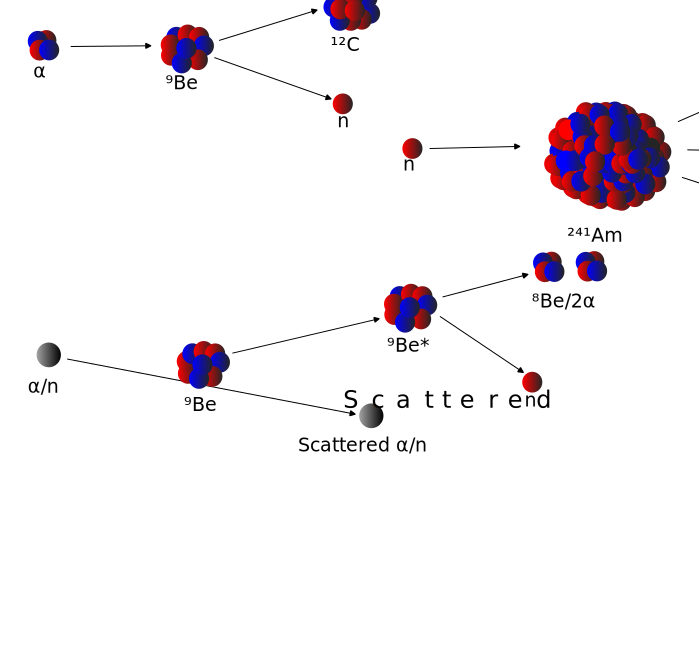
\includegraphics[width=\linewidth]{Fig4.1-AmBe-Processes-landscape}
	\begin{overpic}[width=\linewidth,keepaspectratio]{Fig4.1-AmBe-Processes-landscape}
	\put(-2,32){$^9\text{Be}(\alpha,n)^{12}\text{C}$ --- Q$=+5.702$~MeV}
	\put(60,10){
		$\left.\begin{aligned}
			^9\text{Be}(\alpha,\alpha')\\
			^9\text{Be}(n,n')
		\end{aligned}\right\rbrace$
		$^{9}\text{Be}^* \rightarrow^8\text{Be}/2\alpha+n$
	}
	\put(70,3){--- Q$=-1.665$~MeV}
	\put(60,48){$^{241}\text{Am}(n,f)$ --- Q$\geq200$~MeV}
\end{overpic}
\end{frame}


\begin{frame}\frametitle{Fast reaction}
%REgarding the fast reactions, as we said this can populate excited states of carbon, which then decay emitting 4.4 and 3.2 gammas. These excited states kinematically map to 3 regions, i.e. the higher energy is n0, then n2 and then n2 foing towards 0. Breakup reactions contribute to the 0 to 1 MeV region, and fission neutron can contribute to the entire spectrum range.
\begin{columns}[T]
\begin{column}{0.7\textwidth}
	\centering
	\vspace{-8pt}
	\includegraphics[width=\linewidth]{Fig5.1-GVDZ_resampled.pdf}
AmBe neutron distribution per $^{12}\text{C}$ state [Geiger-Van Der Zwan 1975]
\end{column}
\begin{column}{0.3\textwidth}
	\centering
	\includegraphics[width=\linewidth]{Fig5.2-Levelsout.pdf}
	$^{12}\text{C}$ states - ground, $1^\text{st}$, $2^\text{nd}$ [NNDC]
\end{column}
\end{columns}
\end{frame}

\section*{Current Status}
\begin{frame}\frametitle{Current status}
%Currently, there is an AmBe simulation, whihc simulates $^{241}$Am decay emitting $\alphas$ interacting with beryllium. The issue is, Geant4 lacks differential cross sections and hence crucial features are lacking from the resulting neutron spectrum.
\begin{itemize}
		\item Geant4 has built in example in extended/hadronic/NeutronSource
		\item Simulates $^{241}\text{Am}$ $\alpha$-decay
		\item Lacks differential\\cross sections and\\crucial features
\end{itemize}
	\vspace*{-1.5cm}
	\hspace*{4cm}
	\includegraphics[width=.75\textwidth]{Fig6.1-AmBe_G4Original.pdf}
Geant4 extended/hadronic/NeutronSource example
\centering
%In particular, missing signature peaks of AmBe source, i.e. present the 3.3MeV one, but 5,6.8,7.7 and shoulder at 9.5 is missing
\end{frame}

\section*{Primary Generator}
\begin{frame}\frametitle{Implementation}
%For this reason, we want to make a simulation that is as accurate as possible, efficient, is comprehensive of the reactions occouring and is open-source, so that it can be used for a plethora of applications. For this reason, we chose to directly simulate the neutron and carbon-ion from the fast process, which makes simulations a lot faster considering an emission of 2.27E6 fast neutron per curie per second. This way, we spare about 16300 null events per emerging neutron. We implement this via rejection sampling techniques, adopting integrated cross-sections and differential cross sections in the form of Legendre polynomials from Geiger and van Der Zwan data from 1970 to 1976.
Aim: make the simulation as accurate as possible, efficient, open-source, complete
\begin{itemize}
	\item Simulate $n$ and $^{12}\text{C}$ directly\\
	High activity sources $\Rightarrow$ $2.27\times10^6$ fast neutrons/s/Ci\\
	Simulate one fast neutron per event vs one neutron every $\approx~16300$ events using $\alpha$ decay method
	\item Rejection sampling technique
	\item Integrated cross-section (1970) and Legendre polynomials for differentials (1975,1976 Geiger and Van Der Zwan) for fast neutron reaction
\end{itemize}
\end{frame}


%\begin{frame}\frametitle{Kinematic Lines}
%--What is XS and diff XS? Show difference between XS and diff XS, maybe a snapshot of the adopted data?
%--Kinematic lines are enough to show this
%
% Here showing kinematic lines for the first two states of carbon, clearly showing the angular dependence of the energy of the two reaction products
%\begin{columns}
%	\begin{column}[b]{0.5\linewidth}
%		\vspace*{-1cm}
%		\centering
%		\includegraphics[width=1\linewidth]{9BeA-12Cn-n0.png}
%		\centering
%		\includegraphics[width=\linewidth]{9BeA-12Cn-n2.png}
%	\end{column}
%	\begin{column}[b]{0.5\linewidth}
%		\centering
%		\includegraphics[width=1\linewidth]{9BeA-12Cn-n1.png}
%	\end{column}
%\end{columns}
%\end{frame}


\begin{frame}\frametitle{Differential cross-section contribution}
%Anisotropical approach proposed in 1960s, works pretty well
\begin{columns}
	\begin{column}[b]{0.5\linewidth}
		\centering
		\includegraphics[width=\textwidth]{Fig8.1-AmBeInitialNeutrons100s_isotropic}
		Initial neutrons: without differential cross-sections model
	\end{column}
	\begin{column}[b]{0.5\linewidth}
		\centering
		\includegraphics[width=\textwidth]{Fig8.2-AmBeInitialNeutrons100s_anisotropic}
		Initial neutrons: with differential cross-sections model
	\end{column}
\end{columns}
\end{frame}


\begin{frame}\frametitle{Disadvantages}
\begin{minipage}{\textwidth}
	Differential and Integrated cross section of beryllium-9 break-up not available
	\begin{itemize}
		\item $^{9}\text{Be}(\alpha,\alpha')$ scattering
		\item $^{9}\text{Be}^*$ angular decay information
		\item Other break-up channels more suppressed at interaction energy ($<5$~MeV)\\e.g. $^{9}\text{Be}^* \rightarrow\alpha+ ^{5}\text{He}$
	\end{itemize}
\end{minipage}  
\begin{minipage}{\textwidth}
	\includegraphics[width=\linewidth]{Fig9.1-AmBe-BreakUpProcesses.png}
\end{minipage}  
\end{frame}


\section*{Emerging Neutrons}

\begin{frame}\frametitle{Simulation Results - Emerging Neutrons}
	\centering
	Neutrons emerging from source casing (simulation)
	\centering
	\includegraphics[width=0.9\linewidth]{Fig10.1-EmergingNeutrons20251105.png}
\end{frame}


\begin{frame}\frametitle{Simulation Results - Fission and Break-up Neutrons}
%Here are shown secondary neutrons and fission neutrons emerging from the source casing. Secondaries mostly include (n,2n) reactions. Fission neutrons follow the Watt-fission distribution, have a high Q value that can be in excess of 200~MeV and result in neutron up to 22~MeV being created
	\centering
	Fission and break-up neutrons emerging from the source material
	\centering
	\includegraphics[width=0.9\linewidth]{Fig10-Secondaries_20251020}
\end{frame}


\begin{frame}\frametitle{Simulation Results - AmBe carbon $\gamma$}
%Here we can see that the first and second excited states of carbon are being produced, with Doppler shifting. The production ratio matches cross section values of 26:10:64=n0:n1:n2 wrt to initial neutrons
	\centering
	\includegraphics[width=\linewidth]{Fig12.1-secondaryGammas}
\end{frame}

\section*{Model Comparison}
\begin{frame}\frametitle{Comparison with Geant4 NeutronSource example}
	%And eventually we can see it is very different now, with more defined peaks
	\includegraphics[width=0.9\linewidth]{Fig14.1-EmergingNeutronsvsGeant.pdf}
\end{frame}
\begin{frame}\frametitle{Model comparison}
%spend 2-3 minutes on this
%The simulation matches esperimental results pretty well, especially between 1 and 6 MeV. Below 1 MeV we still have a good match with experimental results, in spite of not simualting any (a,n)/(a,*) reaction. Above 6 MeV, the difference of ouyr yields with experimental ones are due to low accuracy cross sections for the n0 region. Nevertheless, the means match pretty well with experimental results. It is visible it is a great improvement compared to other simulations (Nedis serpent in green and Sources5A in yellow).
	\centering
	Comparison with AmBe standards
	\centering
	\includegraphics[width=.9\linewidth]{Fig13-OverlapLine}
\end{frame}

\section*{Conclusion}
\begin{frame}\frametitle{Conclusion}
\begin{itemize}
	\item Validated AmBe neutron spectrum in Geant4
	\item Correctly reproduced AmBe signature peaks
	\item Implemented 1970 and 1975 Geiger-Van Der Zwan Cross sections (not otherwise present in Geant)
	\item Faster execution than full $^{241}\text{Am}$ $\alpha$-decay chain recreation
	\item Useful for analysis of flux and neutron moderation in various media
	\item Future analysis of neutron moderation in water bath
	%TODO: talk about so what, what to do with this now. Why is this useful
\end{itemize}
\centering
~\\Thank you for listening
\end{frame}


\appendix
\section*{Backup Slides}%Backup slides
\begin{frame}\frametitle{~}
Backup Slides
\end{frame}

\begin{frame}\frametitle{Primary Generator flowchart}
	\centering
	\includegraphics[width=0.7\linewidth]{FigBackup-PrimaryGenerator-v4-crop}
\end{frame}

\begin{frame}\frametitle{Azimuthal emission}
	\centering
	\includegraphics[width=\linewidth]{FigBackup-Azimuthal}
\end{frame}

\begin{frame}\frametitle{Investigation of water bath}
	%AmBe source at centre of 1~m tall, 1~m diameter water tank.\\Fast neutrons are moderated by water. But what is actually happening here?\\
	%\begin{itemize}
	%	\item Mimic neutron moderation in a nuclear reactor
	%	\item Neutron activate samples for undergraduate forensic experiments
	%\end{itemize}
	\begin{itemize}
		\item Source neutron spectrum is known
		\item Source is at centre of 1~m tall, 1~m diameter water tank. The moderation profile is unknown
	\end{itemize}
	%In particular, experimental results from undergraduates disagree with the theroetical data [Lamar Baratta]
\end{frame}

\begin{frame}\frametitle{Two group model}
%NOTE: D is diffusion coefficient, good to know but closely related to the diffusion length via the macroscopic absorbtion cross section
Does it actually agree with the two-group neutron moderation model?
\begin{columns}[T]
	\begin{column}{0.5\textwidth}
		Two group model:
		\[ \Phi_T = \frac{SL_T^2}{4\pi r \overline{D}(L_T^2-\tau_T)}(e^{-r/L_T}-e^{-r/\sqrt{\tau_T}}) \]
		describes thermal neutron diffusion and fast to thermal neutron moderation.\\
		\begin{itemize}
			\item $\tau_T\rightarrow$ (Fast) neutron age
			\item $L_t\rightarrow$ Thermal diffusion length
		\end{itemize}
	\end{column}
	\begin{column}{0.5\textwidth}
		\centering
		\includegraphics[width=\linewidth]{FigBackup-NeutronModeration}
		Neutron moderation $L^2=\frac{1}{6}\overline{r^2}$ [Lamarsh-Baratta 2001]
	\end{column}
\end{columns}
\end{frame}

\begin{frame}\frametitle{Equivalent Dose - Preliminary}
Calculated dose for outgoing $\gamma$ and neutrons from the water bath and verified against experimental\\
Sampling over 0.2~s spectrum
\begin{table}
	\centering
	\begin{tabular}{|c|c|c|}
		\hline
		Particle & Experimental [$\mu\text{Sv/h}$] &  Simulated [$\mu\text{Sv/h}$]\\
		\hline
		$\gamma$ & 1.54 & 8.05 \\
		\hline
		n & 0.8 & 1.68 \\
		\hline
	\end{tabular}
\end{table}
Notes:
\begin{itemize}
	\item Neutrons measured with Nuclear Enterprises NM-2 dose monitor ($BF_3$)
	\item Gammas measured with dose monitor calibrated in the 59-1332~keV range
\end{itemize}
\end{frame}

\end{document}
